\section{Introduksjon}

I de senere år har antall dødsfall som følge av organisert vold økt drastisk
\parencite{davies2022organized}. Samtidig har også finkornet data om
interstatlige konflikter blitt tilgjengelig. Dette åpner for å gjøre
prediksjoner om framtidige dødsfall som gjelder for kortere tidsintervall. Slik
data har blitt satt sammen og vedlikeholdt gjennom \textit{Uppsala Conflict
Data Program (UCDP GED)} \parencite{sundberg2013introducing}. Tidligere studier
på borgerkrig har i stor grad benyttet seg av data aggregert på land og
årsnivå. Dette har vist seg utilstrekkelig får å avdekke faktorer som virker på
lokalnivå og over kortere tidsperioder \parencite{raleigh2010introducing}. Med
UCDP GED-datasettet har vi oppløsningen på enkelthendelser, annotert med
temporale og geografiske metadata. Med høyere oppløsninge på dataene åpner det
seg muligheter for å sammenstille hendelser i borgerkrig med andre lokale data,
både i tid og sted \parencite{eck2012data}. Dette kan gi innsikt i sammenheng
mellom blant annet klimatiske, politiske og økomiske forhold og tap av menneskeliv i
konflikter. Samtidig gir mer finkornet data mulighet til å estimere fremtidige
hendelser for kortere tidsintervall som uker og måneder.

    \begin{figure}[!h]
    \centering
    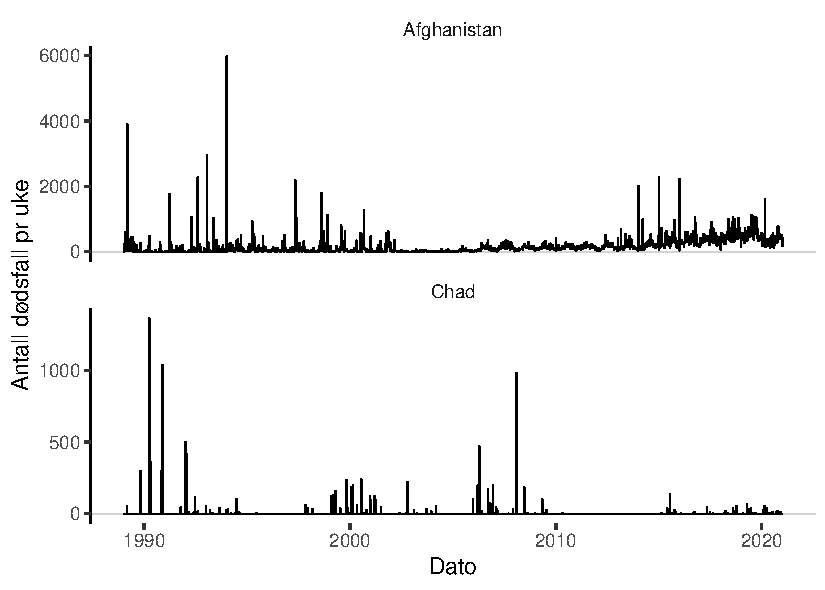
\includegraphics{../img/weekly_deaths}
    \caption{Ukentlig antall drepte i konflikter der staten er en aktør i
        Afghanistan og Chad. Gjennomsnittet er markert med rød linje.}
    \label{fig:weekly_deaths}
    \end{figure}

Samtidig som disse dataene gir nye muligheter for prediksjon og inferens, er
det også utfordringer knyttet til modelleringen av UCDP-dataene. I
\cref{fig:weekly_deaths} kan man se eksempler på ukentlig dødsfall for to
forskjellige land, ett med mange dødsfall pr uke (Afghanistan) og ett hvor det
er lengre tidsintervall mellom uker med dødsfall (Chad). Figuren illustrerer
noen av utfordringene som følger med når man skal modellere på slike data.
For et land som Chad er det overvekt av uker hvor det er 0 dødsfall, såkalt
zero-inflation. Det andre som kommer frem er at variansen er mye høyere enn
forventningen, såkalt overspredning. Videre er responsvariabelen diskret og
nedad begrenset til 0. En sannsynlighetsfordeling som tar høyde for både
zero-inflation og overspredning er nødvendig for å modellere dataene.

I denne oppgaven vil vi se på to mulige modeller for å predikere antall
dødsfall en uke fram i tid i konflikter mellom en statlig og ikke statlig
aktør. Vi vil sammenligne en modell som antar at logaritmen til antall dødsfall
er normalfordelt med en modell hvor vi antar at antall dødsfall er
negativ-binomialfordelt. Vi vil forsøke å vurdere modellene med tanke på hvor
gode de er til å estimere antall dødsfall en uke fram i tid og se hvor gode de
prediktive distribusjonene beskriver de observerte dataene.
 

